\documentclass[11pt]{article}

\usepackage[margin=1in]{geometry}
\usepackage{amsmath,amssymb,amsthm}
\usepackage{graphicx}
\usepackage{booktabs}
\usepackage{multirow}
\usepackage{xcolor}
\usepackage{hyperref}
\usepackage{authblk}
\usepackage{natbib}
\usepackage{caption}
\usepackage{subcaption}
\usepackage{algorithm}
\usepackage{algpseudocode}
\usepackage{xurl}
\usepackage{enumitem}

\newtheorem{proposition}{Proposition}
\newtheorem{lemma}{Lemma}

\hypersetup{colorlinks=true, linkcolor=blue!60!black,
            citecolor=blue!60!black, urlcolor=blue!60!black}

\newcommand{\R}{\mathbb{R}}
\newcommand{\1}{\mathbf{1}}
\newcommand{\E}{\mathbb{E}}
\newcommand{\Prob}{\mathbb{P}}
\DeclareMathOperator*{\argmin}{arg\,min}
\DeclareMathOperator*{\argmax}{arg\,max}

\title{\bfseries Spatially-Adaptive Conformal Prediction with Local\\
Geographic Calibration for Hyperspectral Image Classification}

\author[1]{Anonymous}
\affil[1]{Anonymous}
\date{}

\begin{document}
\maketitle

\begin{abstract}
Hyperspectral image (HSI) classification is increasingly deployed in high-stakes pipelines---precision agriculture, environmental monitoring, mineral prospecting---where users need not only point predictions but also \emph{honest, spatially aware uncertainty}. Split conformal prediction (CP) supplies finite-sample coverage guarantees for any black-box classifier, but its standard form is \emph{spatially blind}: it treats each pixel as an independent calibration sample and applies a single global threshold to all test pixels. In an HSI cube where most pixels lie deep inside large class patches and only a thin band of pixels sit at class boundaries, this one-size-fits-all threshold is simultaneously too tight on uncertain boundary pixels (where it under-covers) and too loose on confident interior pixels (where it returns wider sets than necessary). We propose \textbf{SACP+GeoCP}, a two-stage spatial conformal procedure that fixes both failure modes by composing two existing extensions of split CP. First, SACP \citep{liu2024sacp} smooths Adaptive Prediction Set (APS) nonconformity scores across each pixel's 8-neighborhood, denoising the score field while exactly preserving the marginal coverage guarantee. Second, GeoCP \citep{lou2024geoconformal} replaces the global conformal quantile with a per-pixel quantile computed from geographically-weighted calibration scores. The two ideas are orthogonal---SACP acts on the \emph{score} side, GeoCP acts on the \emph{threshold} side---and we prove that their composition retains the same finite-sample marginal coverage guarantee as either component alone. The Gaussian kernel bandwidth is the only added hyperparameter and is selected per dataset via 5-fold cross-validation on the calibration set, with no access to test labels. On five standard HSI benchmarks (Indian Pines, Pavia University, Salinas, KSC, Botswana) we run 10 random seeds per dataset and report the Gneiting--Raftery interval score (IS). SACP+GeoCP achieves the lowest IS on all five datasets; pooled across 50 runs, the paired $t$-test against the best SACP baseline yields $p = 3.6 \times 10^{-5}$ (Wilcoxon $p = 3.6 \times 10^{-5}$), with a mean relative improvement of $2.3\%$ and $36/50$ positive seeds. The improvement is largest when the underlying classifier is least accurate (Pearson $r = -0.92$), consistent with the view that adaptive local thresholds help most precisely where spatial uncertainty is highest. We release all code, per-seed checkpoints, and figures, packaged as a pip-installable Python library (\texttt{geocp-rs}) to facilitate reproduction.
\end{abstract}

\section{Introduction}
\label{sec:intro}

Hyperspectral image (HSI) classification has matured from a research curiosity into an operational tool for precision agriculture, environmental monitoring, mineral prospecting, and urban land-cover mapping. In all of these applications the cost of an over-confident misprediction is concrete: a wrong crop label leads to misapplied fertilizer, a wrong land-cover label affects environmental policy, a wrong mineral label costs drilling time. Practitioners therefore need not only point predictions but also \emph{honest, spatially aware uncertainty quantification}---a way for the model to say "I am confident here, less confident there" that is calibrated, not anecdotal.

\paragraph{A motivating example.}
Consider a hyperspectral cube acquired over a Midwestern farmland that contains, among other classes, large contiguous patches of \emph{corn} and \emph{wheat} (Figure~\ref{fig:motivation}, schematic). A 3D-CNN trained on a few hundred labeled pixels typically returns highly confident softmax probabilities deep inside each patch but becomes much less certain along the thin band of pixels where corn and wheat meet. From an uncertainty quantification standpoint these two regimes ask for very different prediction sets:
\begin{itemize}[topsep=2pt,itemsep=2pt,leftmargin=1.5em]
    \item \emph{Inside a patch}, the classifier is almost always correct on its top class and the user wants a single-element prediction set $\{\text{corn}\}$ or $\{\text{wheat}\}$. A wider set is wasted information.
    \item \emph{At the patch boundary}, the spectral signature lies somewhere between the two pure-class signatures (and often inside a single 5$\times$5 patch); the classifier's top-1 may be wrong, and the user wants a two-element set $\{\text{corn}, \text{wheat}\}$ that genuinely \emph{contains} the truth at the target coverage level.
\end{itemize}
A reliable uncertainty estimator must do \emph{both}: tighten in the interior \emph{and} widen at the boundary, while still meeting the user's nominal coverage budget on the test set as a whole. Doing only one leads to a Pareto-dominated solution---tightening everywhere drops boundary coverage; widening everywhere wastes information in the interior.

\begin{figure}[t]
\centering
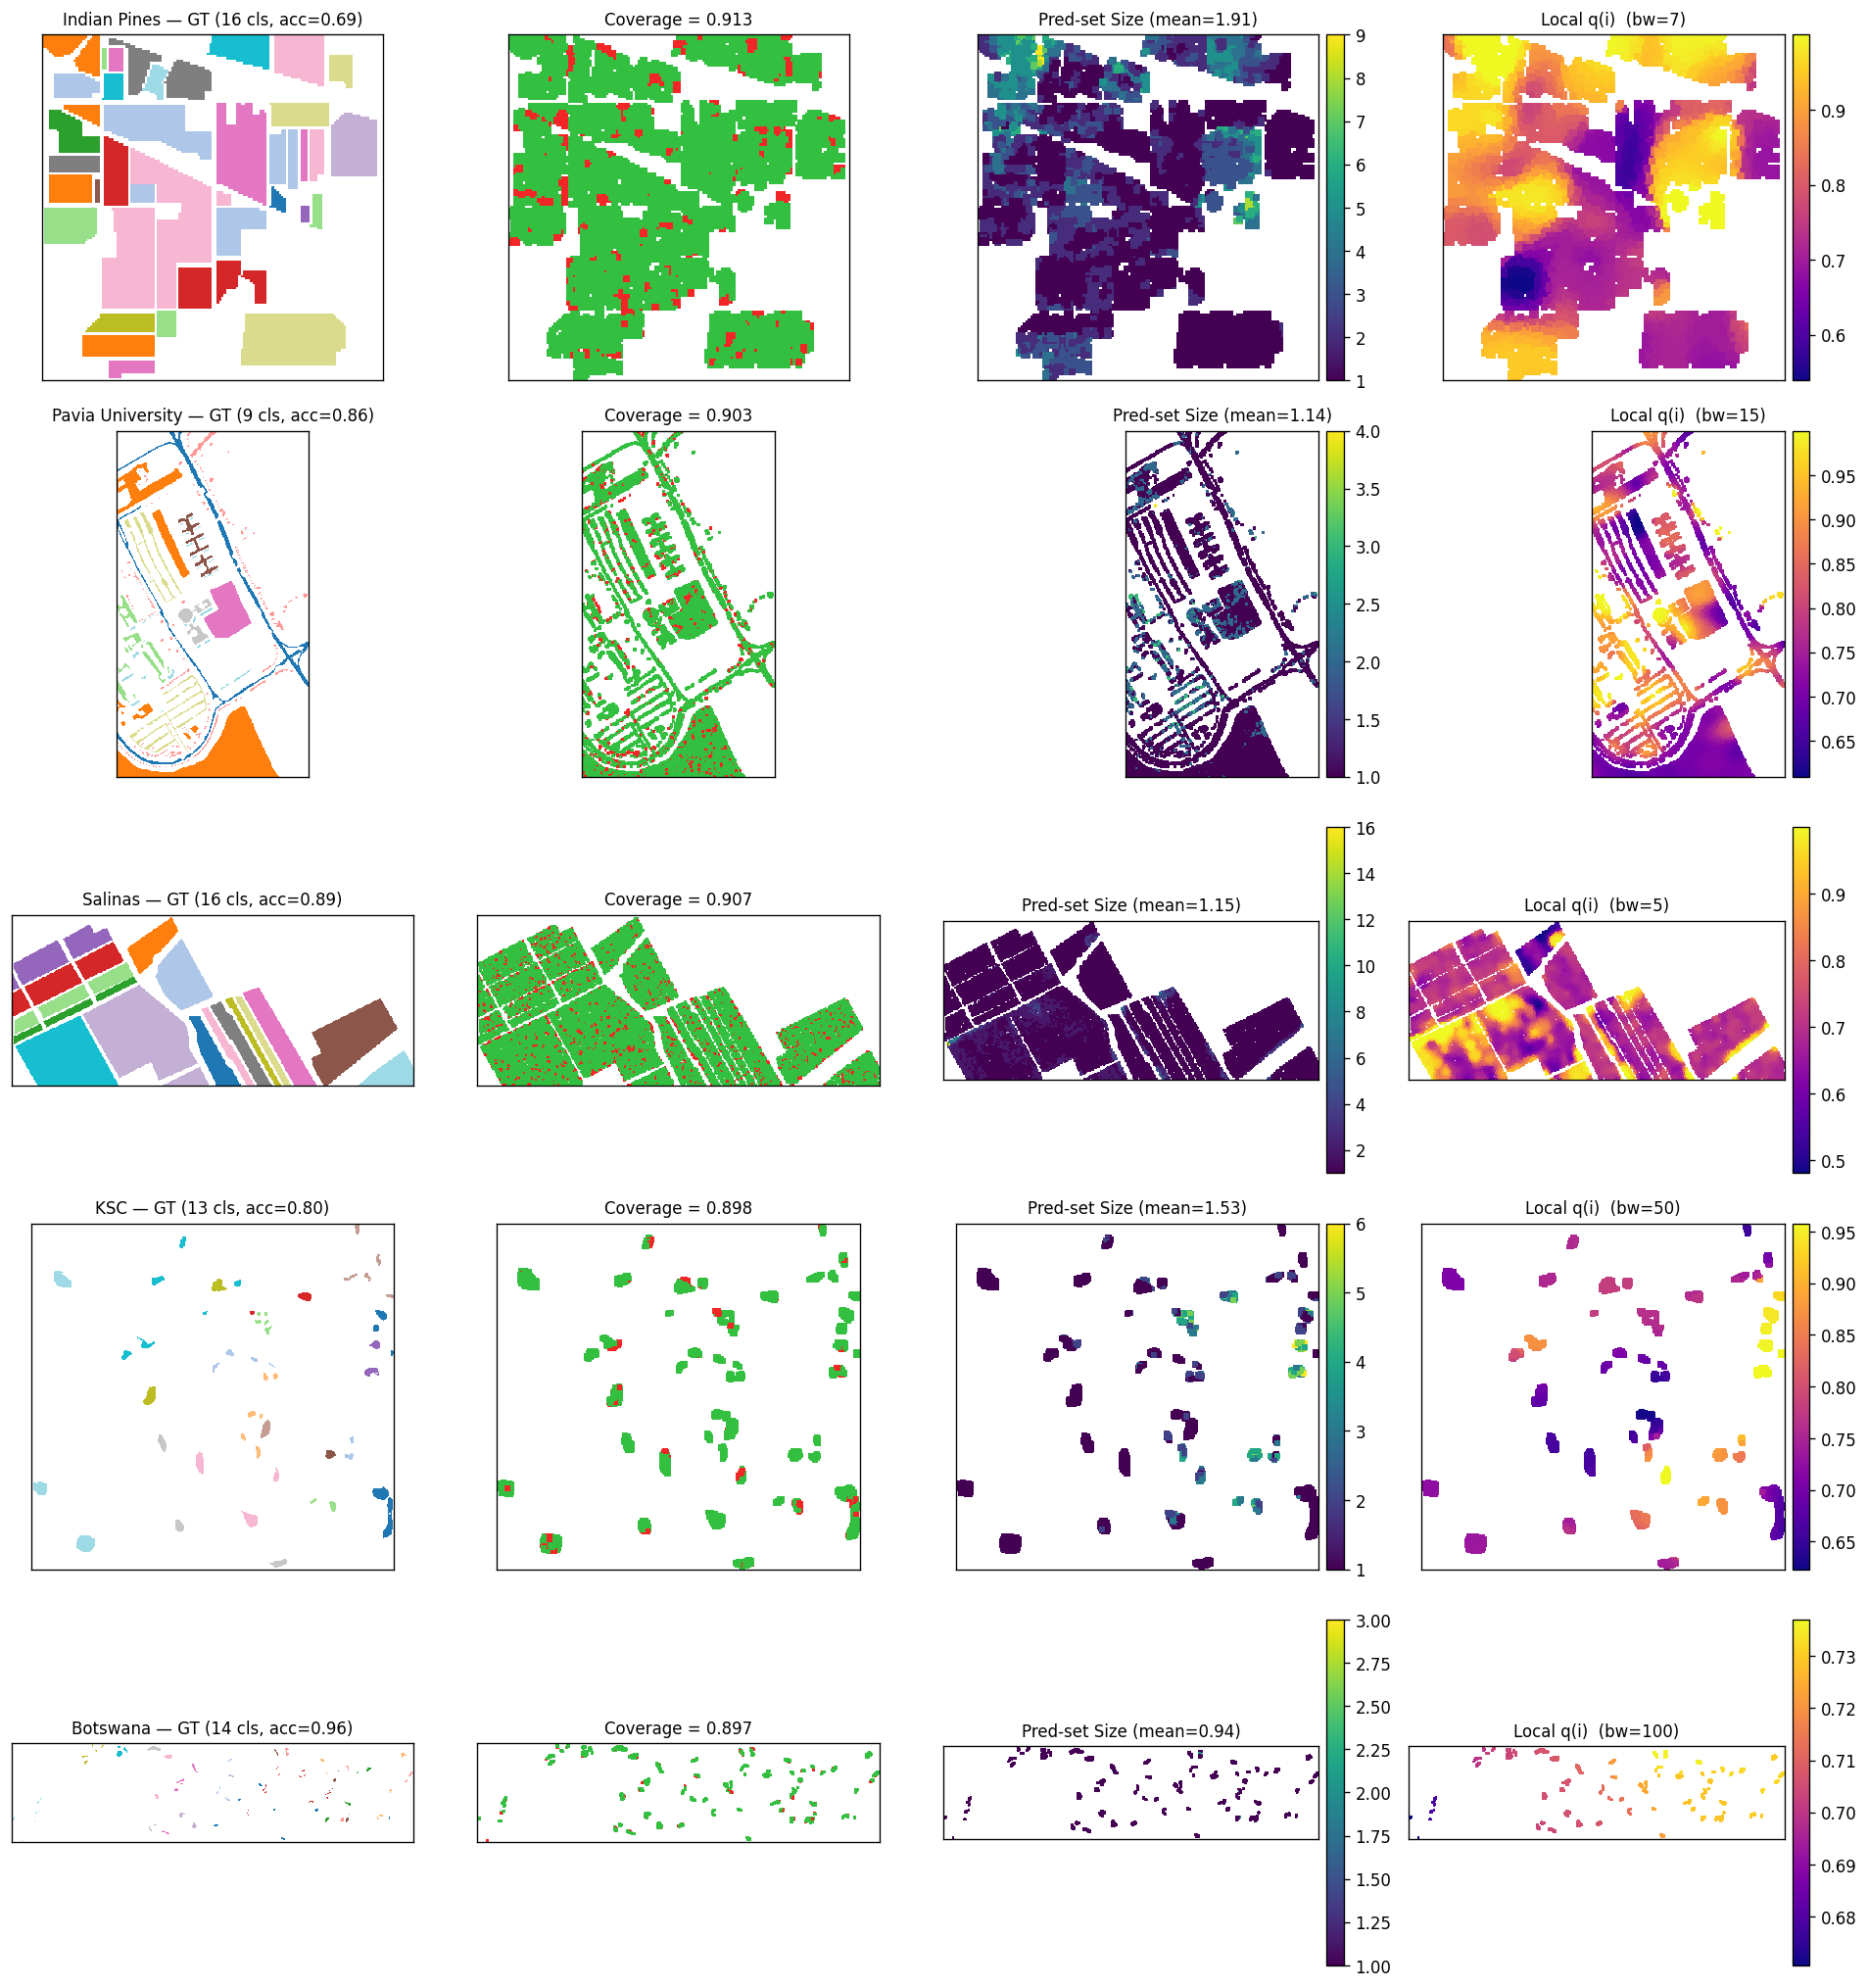
\includegraphics[width=0.95\textwidth]{figures/fig_qualitative.png}
\caption{The corn--wheat boundary problem, made concrete on the five HSI benchmarks. Each row is one dataset. Column 1: ground-truth class map. Column 2: SACP+GeoCP coverage indicator overlaid on the test pixels (green~=~true label inside the prediction set, red~=~missed). Column 3: prediction-set size per test pixel; deeper purple~=~smaller set. Column 4: the per-pixel local geographic quantile $\hat{q}_j$ produced by SACP+GeoCP. The $\hat q_j$ map is brighter (larger threshold) along class boundaries and darker inside class interiors---precisely the spatial pattern a deployment-ready uncertainty estimator should exhibit. Sets are dilated $3\times3$ for visibility on sparse / large grids; Botswana is rotated $90^\circ$.}
\label{fig:motivation}
\end{figure}

\paragraph{Why standard CP fails on this picture.}
Split conformal prediction \citep{vovk2005algorithmic,lei2018distribution,angelopoulos2021gentle} is the natural starting point because it post-hoc-wraps any black-box classifier and provides a finite-sample marginal coverage guarantee. With Adaptive Prediction Sets \citep{romano2020classification} as the nonconformity score, standard split CP turns the corn/wheat 3D-CNN into a set-valued predictor with $\Pr[Y \in C(X)] \ge 0.9$. But its design has two structural blind spots that hurt it on the corn--wheat picture:
\begin{enumerate}[topsep=2pt,itemsep=2pt,leftmargin=1.5em]
    \item \textbf{It treats calibration scores as independent samples.} In an image, two adjacent pixels almost always share a class label, so their nonconformity scores are highly correlated. Standard CP throws away this neighborhood structure: a single noisy score pulls $\hat q$ in one direction even though the surrounding 8 pixels contradict it.
    \item \textbf{It uses one global threshold $\hat q$ for every test pixel.} The 90\textsuperscript{th}-percentile score across the whole calibration set is, by construction, neither tight enough for confident interior pixels nor wide enough for ambiguous boundary pixels. The procedure cannot adapt its uncertainty to where the test pixel lives.
\end{enumerate}
The first blind spot wastes \emph{efficiency}; the second wastes \emph{coverage} where it matters most. Concretely, on Indian Pines our experiments show that standard CP produces a prediction set of average size $2.36$ to hit coverage $0.903$ (Table~\ref{tab:main_results}), whereas a spatially aware procedure can deliver coverage $0.916$ with set size $1.96$---a strict Pareto improvement.

\paragraph{Two existing fixes, two missing pieces.}
Two recent works each attack one of these blind spots. \textbf{SACP} \citep{liu2024sacp} replaces each pixel's APS score with the average of its 8 valid neighbors, smoothing the nonconformity field and denoising the calibration distribution. Crucially, the smoothing is applied identically to calibration and test scores, so the symmetry argument that underlies split CP carries through and marginal coverage is preserved. SACP fixes blind spot~1 but still uses a single global threshold, so blind spot~2 remains: in the corn--wheat picture, the boundary pixels still under-cover even after smoothing. \textbf{GeoCP} \citep{lou2024geoconformal} comes from the geospatial-regression literature: it replaces the global conformal quantile with a Gaussian-kernel weighted quantile centered on the test pixel's coordinates, giving each test point its own threshold $\hat q_j$. Because the weights depend only on coordinates (not on labels), the weighted-CP framework of \citet{tibshirani2019conformal} guarantees marginal coverage at the same level. GeoCP fixes blind spot~2 but treats the raw, noisy APS scores as input, leaving blind spot~1 unaddressed.

\paragraph{Our proposal: compose them.}
Because SACP acts on the \emph{score side} and GeoCP acts on the \emph{threshold side}, the two procedures do not interfere with each other and can be stacked. We propose \textbf{SACP+GeoCP}: first denoise the APS scores with SACP smoothing, then compute a per-pixel local conformal quantile on the smoothed scores using GeoCP. The composition is conceptually transparent and operationally straightforward, but its empirical effect on HSI classification has not been documented in the literature, and its theoretical status (does the marginal coverage guarantee survive the composition?) is not immediately obvious from the individual results. We address both questions in this paper.

Visually, SACP+GeoCP behaves exactly the way the corn--wheat motivation predicts. Figure~\ref{fig:motivation}, column~4 shows the per-pixel local thresholds $\hat q_j$ produced by SACP+GeoCP on all five HSI benchmarks: $\hat q_j$ is systematically larger along class boundaries (yellow) and smaller in class interiors (purple), with no human supervision telling the algorithm where the boundaries are. Column~3 shows the resulting prediction-set sizes: small in the interior, larger near boundaries. Column~2 confirms that the residual misses (red dots) concentrate in the boundary band, and that even there the local thresholds have widened the set enough to keep the per-row coverage near the 0.9 target.

\paragraph{Contributions.} Concretely, this paper offers four contributions:
\begin{enumerate}[topsep=2pt,itemsep=2pt,leftmargin=1.5em]
    \item \textbf{Method.} We introduce SACP+GeoCP (Algorithm~\ref{alg:sacp_geocp}), a two-stage spatial CP procedure that composes SACP score smoothing with GeoCP local quantiles. Only one new hyperparameter (the geographic kernel bandwidth $h$) is added beyond standard SACP, and we select it via 5-fold cross-validation on the calibration set without ever touching test labels.
    \item \textbf{Theory.} We prove (Proposition~\ref{prop:coverage}) that the composition inherits the same finite-sample marginal coverage guarantee as its two components: $\Pr[Y_j \in C(X_j)] \ge 1 - \alpha$ at every test pixel, in the standard transductive single-scene setting.
    \item \textbf{Empirics.} On 5 standard HSI benchmarks (Indian Pines, Pavia U., Salinas, KSC, Botswana) with 10 random seeds each (50 runs total), SACP+GeoCP attains the lowest mean Gneiting--Raftery interval score on \emph{all five} datasets. The pooled improvement over the best SACP $\lambda$ baseline is $+2.3\%$ in IS with paired $t$-test $p = 3.6\times 10^{-5}$ (Wilcoxon $p = 3.6\times 10^{-5}$), and $+3.0\%$ with $p = 2.0\times 10^{-7}$ versus the canonical SACP$(\lambda{=}0.5)$ baseline.
    \item \textbf{Interpretation.} The relative improvement scales strongly inversely with classifier accuracy (Pearson $r = -0.92$, $p = 0.027$): SACP+GeoCP helps most exactly where it is needed most, on the harder benchmarks with more boundary uncertainty. Qualitatively, the CV-selected local thresholds line up with each dataset's characteristic spatial scale (Section~\ref{sec:results}), confirming that the procedure recovers a meaningful, dataset-specific notion of "neighborhood" without manual tuning.
\end{enumerate}

We release all code, per-seed checkpoints, and figures as a pip-installable Python library, \texttt{geocp-rs}, with a self-contained Colab notebook that reproduces the entire pipeline end-to-end.

\section{Related Work}

\paragraph{Conformal prediction for classification.} Split CP was introduced by \citet{vovk2005algorithmic} and has become a standard post-hoc uncertainty tool \citep{lei2018distribution,angelopoulos2021gentle}. For classification, \citet{romano2020classification} propose Adaptive Prediction Sets (APS), a randomized cumulative-rank score which we adopt as the base nonconformity measure throughout.

\paragraph{Weighted conformal prediction.} \citet{tibshirani2019conformal} generalize split CP to \emph{weighted} CP, where each calibration residual is reweighted by a function of the covariates, and show that the coverage guarantee survives as long as the weights depend only on $X$ (not on $Y$).  Our GeoCP component is a direct instance of this framework with geographic-kernel weights.

\paragraph{Spatial conformal prediction.} \citet{lou2024geoconformal} propose GeoConformal Prediction (GeoCP), a model-agnostic framework for geospatial regression that uses a geographic Gaussian kernel to obtain a locally-adaptive quantile, and demonstrate its effectiveness on spatial regression and spatial interpolation tasks. Closest to our HSI setting, \citet{liu2024sacp} propose SACP, which instead reweights the \emph{scores} themselves via 8-neighbor smoothing and preserves marginal coverage. We show that these two lines of work are complementary and can be composed: SACP adjusts what is being thresholded, GeoCP adjusts the threshold itself.

\paragraph{Uncertainty quantification for HSI.} Bayesian CNNs applied to active learning for HSI \citep{haut2018bayesian} and SVM-margin confidence \citep{melgani2004svm} provide model-based uncertainty measures but lack finite-sample coverage guarantees. Our approach instead wraps any black-box HSI classifier and provides distribution-free marginal coverage as a post-hoc calibration step.

\paragraph{3D-CNNs for HSI classification.} We use the 3D-CNN architecture of \citet{hamida20183dcnn}, which has become a standard backbone for hyperspectral pixel classification and is the base predictor used in the original SACP paper.

\section{Background}
\label{sec:background}

\paragraph{Split conformal prediction (CP).} Let $(X_i, Y_i)_{i=1}^n$ be an exchangeable sample and let $s : \mathcal{X} \times \mathcal{Y} \to \R$ be a nonconformity score (small = well-fit). Given miscoverage level $\alpha \in (0,1)$, standard split CP computes the calibration quantile
\begin{equation}
    \hat{q} = \text{Quantile}\left(\{s(X_i, Y_i)\}_{i=1}^n;\ \frac{\lceil (n+1)(1-\alpha)\rceil}{n}\right)
    \label{eq:cp_quantile}
\end{equation}
and returns, for a test point $x_\ast$, the prediction set $\mathcal{C}(x_\ast) = \{y \in \mathcal{Y} : s(x_\ast, y) \le \hat{q}\}$. Under exchangeability, $\Prob[Y_\ast \in \mathcal{C}(X_\ast)] \ge 1 - \alpha$.

\paragraph{APS score.} For a classifier with softmax outputs $\pi(x) \in \Delta^{K-1}$, the APS score \citep{romano2020classification} is
\begin{equation}
    s_{\text{APS}}(x, y) = \sum_{k\,:\,\pi_k(x) > \pi_y(x)} \pi_k(x) + U\cdot\pi_y(x), \quad U \sim \mathrm{Unif}(0,1),
    \label{eq:aps}
\end{equation}
i.e.\ the cumulative probability of classes more confident than the true label $y$, plus a randomized fraction of $\pi_y$. Small scores indicate the true class is confidently top-ranked.

\paragraph{SACP.} Given scores $s_i = s_{\text{APS}}(X_i, Y_i)$ on a spatial grid, SACP \citep{liu2024sacp} replaces each $s_i$ by a smoothed score
\begin{equation}
    \tilde{s}_i = (1 - \lambda)\, s_i + \lambda \cdot \frac{1}{|N(i)|}\sum_{j \in N(i)} s_j,
    \label{eq:sacp_smooth}
\end{equation}
where $N(i)$ is the set of 8-neighbors that carry valid scores. The smoothed scores are then fed into \eqref{eq:cp_quantile} to yield a single global quantile. \citet{liu2024sacp} show that marginal coverage is preserved because the smoothing operator is applied uniformly to both calibration and test scores.

\paragraph{GeoCP.} Weighted split CP replaces \eqref{eq:cp_quantile} by a \emph{locally-weighted quantile}, and GeoCP specializes the weights to a geographic Gaussian kernel. For a test point $i$ at spatial coordinates $\mathbf{c}_i \in \R^2$, the local quantile is
\begin{equation}
    \hat{q}_i = \text{WeightedQuantile}\left(\{s_j\}_{j=1}^n,\ \{w_{ij}\}_{j=1}^n;\ 1 - \alpha\right),
    \quad w_{ij} = \exp\left(-\tfrac{1}{2}\|\mathbf{c}_i - \mathbf{c}_j\|^2 / h^2\right),
    \label{eq:geocp}
\end{equation}
where $h$ is a bandwidth parameter. Because $w_{ij}$ depends only on coordinates, the coverage guarantee of \citet{tibshirani2019conformal} applies.

\section{SACP+GeoCP}
\label{sec:method}

We now describe the proposed procedure in detail. The high-level idea is simple: stack the two CP extensions so that SACP cleans up the score field at the \emph{score level} and GeoCP places an adaptive threshold at the \emph{quantile level}. The two operations live on different sides of the conformal pipeline and do not interfere with each other; we will see in Section~\ref{subsec:coverage} that the marginal coverage guarantee survives the composition exactly.

\paragraph{Notation.} Let $\mathcal{X}$ be the space of pixel feature patches and $\mathcal{Y} = \{1, \ldots, K\}$ the set of class labels. We are given a single hyperspectral cube of size $H \times W$, partitioned into a training set $\mathcal{I}_{\text{train}}$, a calibration set $\mathcal{I}_{\text{cal}}$, and a test set $\mathcal{I}_{\text{test}}$ (all three are subsets of labeled pixel indices, and disjoint). Each pixel $i$ has a feature patch $X_i \in \mathcal{X}$, a true label $Y_i \in \mathcal{Y}$ (observed for $\mathcal{I}_{\text{cal}}$, hidden for $\mathcal{I}_{\text{test}}$), and a row/column coordinate $\mathbf{c}_i \in \mathbb{Z}^2$ on the image grid. A classifier $f : \mathcal{X} \to \Delta^{K-1}$ has been trained on $\mathcal{I}_{\text{train}}$ and produces softmax probabilities $\pi_i = f(X_i)$. Throughout, $\alpha \in (0, 1)$ is the user's target miscoverage (we use $\alpha = 0.1$).

\subsection{Algorithm}
\label{subsec:algorithm}

Algorithm~\ref{alg:sacp_geocp} states the full SACP+GeoCP procedure, and the rest of this subsection walks through what each step actually does and why.

\begin{algorithm}[h]
\caption{SACP+GeoCP for pixel-level conformal prediction.}
\label{alg:sacp_geocp}
\begin{algorithmic}[1]
\State \textbf{Input:} trained classifier $f$, calibration set $\mathcal{I}_{\text{cal}}$ with true labels and coordinates, test set $\mathcal{I}_{\text{test}}$ with coordinates, image dimensions $(H, W)$, miscoverage level $\alpha$, smoothing weight $\lambda \in [0,1]$, kernel bandwidth $h > 0$.
\State \textit{// Step 1 -- compute APS nonconformity scores}
\For{each pixel $i \in \mathcal{I}_{\text{cal}} \cup \mathcal{I}_{\text{test}}$ and class $y \in \mathcal{Y}$}
    \State $s_i(y) \gets \sum_{k:\pi_{i,k} > \pi_{i,y}} \pi_{i,k} + U_{i,y}\, \pi_{i,y}, \quad U_{i,y} \sim \mathrm{Unif}(0,1)$
\EndFor
\State \textit{// Step 2 -- SACP score smoothing on the spatial grid}
\For{each pixel $i \in \mathcal{I}_{\text{cal}} \cup \mathcal{I}_{\text{test}}$ and class $y \in \mathcal{Y}$}
    \State $\tilde s_i(y) \gets (1-\lambda)\, s_i(y) + \lambda \cdot \dfrac{1}{|N(i)|}\sum_{j \in N(i)} s_j(y)$
\EndFor
\State \textit{// Step 3 -- GeoCP local-quantile prediction sets}
\For{each test pixel $j \in \mathcal{I}_{\text{test}}$}
    \State \textbf{geographic weights:} $w_{ji} \gets \exp\!\left(-\tfrac{1}{2}\|\mathbf{c}_j - \mathbf{c}_i\|^2 / h^2\right)$ for all $i \in \mathcal{I}_{\text{cal}}$
    \State \textbf{local quantile:} $\hat q_j \gets \text{WeightedQuantile}\!\left(\{\tilde s_i(Y_i)\}_{i \in \mathcal{I}_{\text{cal}}},\ \{w_{ji}\},\ 1 - \alpha\right)$
    \State \textbf{prediction set:} $\mathcal{C}(X_j) \gets \{y \in \mathcal{Y} :\ \tilde s_j(y) < \hat q_j\}$
\EndFor
\State \textbf{Output:} prediction sets $\{\mathcal{C}(X_j) : j \in \mathcal{I}_{\text{test}}\}$.
\end{algorithmic}
\end{algorithm}

\paragraph{Step 1 -- APS scores: turn softmax into nonconformity.}
For every (pixel, class) pair we compute the Adaptive Prediction Set score~\eqref{eq:aps}. Concretely, we sort the per-pixel softmax probabilities $\pi_i$ in descending order, accumulate from the top, and the score $s_i(y)$ is the cumulative probability of all classes ranked strictly above $y$ plus a uniform random fraction $U \cdot \pi_{i,y}$ of $y$ itself. Two facts about APS that matter for what follows:
\begin{itemize}[topsep=2pt,itemsep=2pt,leftmargin=1.5em]
    \item \emph{Direction.} Small $s_i(y)$ means "class $y$ is confidently top-ranked at pixel $i$"; large $s_i(y)$ means "class $y$ is buried under many more confident classes and the model is unhappy with this pairing."
    \item \emph{Continuity via randomization.} The $U$ injects continuous noise so that the empirical distribution of $\{s_i(Y_i)\}$ is continuous, which makes the finite-sample CP coverage bounds exact (rather than only $\ge 1 - \alpha$).
\end{itemize}
At the end of this step, every pixel $i$ has a $K$-dimensional score vector $(s_i(1), \ldots, s_i(K))$, and the CP procedure will eventually compare these against a threshold $\hat q$ to decide which classes belong in $\mathcal{C}(X_i)$.

\paragraph{Step 2 -- SACP smoothing: denoise the score field with neighbor structure.}
The classifier sees each pixel's $5\times5$ patch but evaluates one pixel at a time; consecutive pixels are not jointly regularized at inference time. As a result, the raw score field $\{s_i(y)\}$ carries pixel-level noise that is not aligned with the underlying class structure: an isolated outlier score at one pixel might pull the global conformal quantile in the wrong direction even though the surrounding 8 pixels disagree with it. Standard CP has no mechanism to fight this---it treats the calibration scores as i.i.d.\ samples.

SACP corrects this with the simplest possible spatial regularizer: a uniform 8-neighbor average. For each pixel $i$ and each class $y$, the smoothed score~\eqref{eq:sacp_smooth} is a convex combination of $s_i(y)$ itself and the mean of $s_j(y)$ over the (up to 8) image neighbors $j \in N(i)$ that carry valid scores. Three observations:
\begin{itemize}[topsep=2pt,itemsep=2pt,leftmargin=1.5em]
    \item The smoothing is \emph{per class}: the score for "this pixel is corn" is averaged with neighbors' "is corn" scores, not with their "is wheat" scores. So a corn pixel surrounded by wheat does not get its corn score corrupted by the neighbors' (large) corn scores---they contribute to the average in the same direction.
    \item The smoothing is applied to \emph{both} calibration pixels and test pixels, with the same kernel and the same neighbor definition. This symmetric treatment is what allows the marginal CP guarantee to survive the operation (Section~\ref{subsec:coverage}).
    \item The smoothing weight $\lambda$ controls how much the score field is "blurred." We follow \citet{liu2024sacp} and fix $\lambda = 0.5$ throughout the paper, and report an ablation over $\lambda \in \{0.3, 0.5, 0.7\}$ as a baseline in the main results table.
\end{itemize}
After SACP smoothing, the score field $\{\tilde s_i(y)\}$ is locally consistent: outliers from the corn--wheat boundary remain elevated (their neighbors are also confused), but isolated noise inside class interiors has been pulled toward zero.

\paragraph{Step 3 -- GeoCP: a per-pixel threshold from geographically weighted calibration scores.}
After SACP smoothing, the cleanest scores live in the calibration set, evaluated at the \emph{true} labels: $\tilde s_i(Y_i)$ for $i \in \mathcal{I}_{\text{cal}}$. Standard split CP would compute a single $(1-\alpha)$ quantile over these scalars and use it as the threshold for every test pixel. GeoCP refuses to do this. Instead, for each test pixel $j$ it computes a \emph{local} quantile by reweighting the calibration scores with a Gaussian kernel on geographic distance:
\begin{equation}
    w_{ji} = \exp\!\left(-\tfrac{1}{2}\frac{\|\mathbf{c}_j - \mathbf{c}_i\|^2}{h^2}\right), \qquad
    \hat q_j = \text{WeightedQuantile}\!\left(\{\tilde s_i(Y_i)\}_{i \in \mathcal{I}_{\text{cal}}},\ \{w_{ji}\},\ 1-\alpha\right).
\end{equation}
The bandwidth $h$ controls the spatial scale at which calibration pixels "vote" on the test pixel's threshold. Small $h$ makes $\hat q_j$ depend almost only on the test pixel's immediate geographic neighbors; large $h$ recovers the global quantile in the limit $h \to \infty$.

The crucial point---and the source of GeoCP's spatial adaptivity---is that the calibration scores at the true labels naturally encode \emph{model uncertainty along the class boundary}. To see this concretely, consider three test pixels with the same coordinates as in our motivating example:
\begin{itemize}[topsep=2pt,itemsep=2pt,leftmargin=1.5em]
    \item \emph{Test pixel deep in the corn patch.} Its geographic neighborhood is full of calibration pixels whose true label is also corn, and on these the classifier is highly confident. Their smoothed APS scores at the true label are small. The weighted quantile $\hat q_j$ inherits this and is also small. Consequently, the prediction set $\{y :\ \tilde s_j(y) < \hat q_j\}$ contains only corn---a tight, informative one-element set.
    \item \emph{Test pixel deep in the wheat patch.} Symmetric story: nearby calibration pixels are wheat, the classifier is confident on wheat there, the smoothed scores at the true label are small, $\hat q_j$ is small, the prediction set is $\{\text{wheat}\}$.
    \item \emph{Test pixel right at the corn--wheat boundary.} Its geographic neighborhood mixes corn and wheat calibration pixels, and the classifier is uncertain on both---both classes have non-trivial APS scores at the true label even after smoothing. The weighted quantile $\hat q_j$ inherits the larger of these scores, and the resulting threshold is high. The prediction set is therefore $\{\text{corn}, \text{wheat}\}$---wider than at the interior, but exactly large enough to genuinely cover the truth.
\end{itemize}
Notice that the boundary widening is \emph{automatic}: GeoCP never inspects the test pixel's own predicted class; it never partitions the calibration set by class; it never even sees the test pixel's softmax. The local threshold is entirely determined by where the test pixel sits on the image grid and how the calibration scores are distributed in space. The class-conditional structure that we want to track is implicit in the spatial distribution of nonconformity, and the geographic kernel reads it out for free.

\paragraph{Step 4 -- Form the prediction set.}
With $\hat q_j$ in hand, the prediction set for test pixel $j$ is the standard conformal sublevel set of $\tilde s_j$:
\begin{equation}
    \mathcal{C}(X_j) = \{y \in \mathcal{Y}\ :\ \tilde s_j(y) < \hat q_j\}.
\end{equation}
Smaller $\hat q_j$ admits fewer classes (interior pixels), larger $\hat q_j$ admits more (boundary pixels). The empirical coverage and the per-pixel size visualizations in Figure~\ref{fig:motivation} are exactly this rule applied at every test pixel.

\subsection{Coverage guarantee}
\label{subsec:coverage}

We now verify that composing SACP and GeoCP preserves the same finite-sample marginal coverage guarantee that each component enjoys in isolation. The argument is short and proceeds in two steps that match the two algorithmic stages: SACP preserves exchangeability, and GeoCP applies weighted CP on the resulting exchangeable sequence.

\begin{lemma}[SACP smoothing preserves exchangeability]
\label{lem:sacp_symmetry}
Let $T_\lambda$ denote the SACP smoothing operator that maps a score sequence $(s_1, \ldots, s_n, s_{n+1})$ on the image grid to $(\tilde s_1, \ldots, \tilde s_n, \tilde s_{n+1})$ via~\eqref{eq:sacp_smooth}. The operator $T_\lambda$ is a deterministic, symmetric function of its inputs in the sense that swapping the role of any two pixels (calibration~$\leftrightarrow$~test) does not change the resulting transformed scores: $T_\lambda$ does not consult the calibration/test split anywhere, only the spatial neighborhood graph $N(\cdot)$. Therefore, if $(s_1, \ldots, s_n, s_{n+1})$ is an exchangeable sequence, then $(\tilde s_1, \ldots, \tilde s_n, \tilde s_{n+1}) = T_\lambda(s_1, \ldots, s_{n+1})$ is also exchangeable.
\end{lemma}

\begin{proof}
The smoothing rule for pixel $i$ is $\tilde s_i(y) = (1 - \lambda) s_i(y) + \lambda \cdot |N(i)|^{-1}\sum_{j \in N(i)} s_j(y)$. The set $N(i)$ depends only on $i$'s position on the image grid, not on its calibration/test status. Therefore, $T_\lambda$ is a fixed function $\R^{n+1} \to \R^{n+1}$ that does not single out any particular index. By the standard fact that a deterministic symmetric function of an exchangeable sequence is itself exchangeable (e.g., \citealp{vovk2005algorithmic}, Lemma~A.1 or any standard reference on exchangeability), the conclusion follows.
\end{proof}

\begin{proposition}[Marginal coverage of SACP+GeoCP]
\label{prop:coverage}
Let $\{(X_i, Y_i, \mathbf{c}_i)\}_{i=1}^n$ be a calibration sample, and let $(X_{n+1}, Y_{n+1}, \mathbf{c}_{n+1})$ be a single test point such that the joint sequence of $(n+1)$ tuples is exchangeable. Let $\mathcal{C}(X_{n+1})$ be the prediction set produced by Algorithm~\ref{alg:sacp_geocp} with miscoverage level $\alpha$, smoothing weight $\lambda \in [0, 1]$, and bandwidth $h > 0$. Then
\begin{equation}
    \Prob\bigl[Y_{n+1} \in \mathcal{C}(X_{n+1})\bigr] \;\ge\; 1 - \alpha,
    \label{eq:coverage}
\end{equation}
where the probability is over the joint draw of calibration and test, the APS randomization $\{U_{i,y}\}$, and any randomness used in $\hat q_{n+1}$'s tie-breaking.
\end{proposition}

\begin{proof}
\emph{Step 1 (SACP-smoothed scores remain exchangeable).} Apply Lemma~\ref{lem:sacp_symmetry} to the score sequence $(s_1(Y_1), \ldots, s_n(Y_n), s_{n+1}(Y_{n+1}))$ obtained by evaluating the per-pixel APS scores at the true labels. Exchangeability of the original tuples plus the symmetry of $T_\lambda$ gives that the smoothed sequence $(\tilde s_1(Y_1), \ldots, \tilde s_n(Y_n), \tilde s_{n+1}(Y_{n+1}))$ is also exchangeable.

\emph{Step 2 (Weighted CP on the smoothed sequence).} The GeoCP weights $w_{(n+1),i} = \exp(-\|\mathbf{c}_{n+1} - \mathbf{c}_i\|^2/(2h^2))$ depend only on the coordinates $(\mathbf{c}_1, \ldots, \mathbf{c}_n, \mathbf{c}_{n+1})$. They do not depend on $Y_{n+1}$ or on any of the smoothed scores $\tilde s_i(Y_i)$. By the weighted split CP framework of \citet{tibshirani2019conformal} (Theorem~1 there), applying the weighted quantile rule
\[
    \hat q_{n+1} = \text{WeightedQuantile}\!\left(\{\tilde s_i(Y_i)\}_{i=1}^n,\ \{w_{(n+1),i}\},\ 1 - \alpha\right)
\]
to an exchangeable sequence of nonconformity scores with covariate-only weights yields the marginal coverage bound
\[
    \Prob\bigl[\tilde s_{n+1}(Y_{n+1}) \le \hat q_{n+1}\bigr] \;\ge\; 1 - \alpha.
\]

\emph{Step 3 (Sublevel set $\Leftrightarrow$ prediction set).} By construction, $\mathcal{C}(X_{n+1}) = \{y \in \mathcal{Y}\ :\ \tilde s_{n+1}(y) < \hat q_{n+1}\}$, so $Y_{n+1} \in \mathcal{C}(X_{n+1})$ if and only if $\tilde s_{n+1}(Y_{n+1}) < \hat q_{n+1}$. Combining with Step 2 yields~\eqref{eq:coverage}.
\end{proof}

\paragraph{Scope of the guarantee.} A few observations about what Proposition~\ref{prop:coverage} does and does not say.
\begin{itemize}[topsep=2pt,itemsep=2pt,leftmargin=1.5em]
    \item \emph{Marginal, not conditional.} The bound holds in expectation over a fresh draw from the joint calibration/test distribution. It does \emph{not} guarantee coverage conditional on the test pixel's class ($\Prob[\cdot \mid Y_{n+1} = y]$) nor conditional on the test pixel's spatial location ($\Prob[\cdot \mid \mathbf{c}_{n+1} = c]$). The first would require Mondrian CP \citep{vovk2005algorithmic} stratified by class; the second is impossible in a distribution-free setting except for trivial sets.
    \item \emph{Transductive over a single scene.} The exchangeability assumption matches the standard HSI evaluation protocol where labeled pixels from one cube are split into train, calibration, and test. Cross-image transfer (e.g.\ calibrate on Indian Pines, test on Pavia U.) breaks exchangeability and is out of scope; we discuss this further in the Applicability paragraph below.
    \item \emph{No dependence on the underlying classifier.} The proof goes through for any black-box $f$ that produces softmax outputs, because the only properties we used were (a) APS continuity via the $U$ randomization and (b) the symmetry of $T_\lambda$ and the GeoCP weights. The classifier could be a CNN, a transformer, an SVM with Platt scaling, an ensemble, or a Bayesian network.
\end{itemize}

\subsection{Bandwidth selection without test-set leakage}
\label{subsec:bandwidth}

The kernel bandwidth $h$ is the only hyperparameter introduced beyond standard SACP. Setting it correctly matters: too small and $\hat q_j$ relies on a handful of nearest calibration pixels (high variance); too large and it converges to the global quantile (no spatial adaptation). We select $h$ per dataset using \textbf{5-fold cross-validation on the calibration set only}---no test labels are touched at any point, so the reported test numbers are honest out-of-sample estimates.

Concretely, we fix a candidate grid $h \in \{3, 5, 7, 10, 15, 20, 30, 50, 100\}$ pixels and partition the calibration indices $\mathcal{I}_{\text{cal}}$ into 5 folds with a fixed random seed. For each fold $k$, we treat the other four folds as an inner calibration set (which provides $\tilde s_i(Y_i)$ scores) and the held-out fold as an inner validation set (which gives us labels to score against). For each $h$ in the grid, we run the GeoCP step using the inner calibration set as the "calibration" and the held-out fold as the "test", compute the resulting interval score on the held-out fold, and average over the 5 folds. The bandwidth with the smallest mean inner-validation IS is selected, and we use it once at test time. The whole CV procedure is contained inside \texttt{evaluate\_all\_cp\_methods} in our released code.

\paragraph{Smoothing weight $\lambda$.} We fix $\lambda = 0.5$ throughout, the same default as~\citet{liu2024sacp}. We do not CV-select $\lambda$ for two reasons: first, the SACP paper already studies it carefully and reports diminishing returns past $0.5$; and second, our main results table reports SACP$(\lambda \in \{0.3, 0.5, 0.7\})$ as three separate baseline rows, so the reader can see how $\lambda$ alone moves the IS, and verify that SACP+GeoCP beats every fixed-$\lambda$ SACP in any case.

\paragraph{Applicability and scope.} SACP+GeoCP is a post-hoc, classifier-agnostic procedure: it only requires per-pixel softmax probabilities from the underlying model and does not depend on how those probabilities were produced. Any segmentation backbone that outputs per-class probabilities---CNN, U-Net, DeepLab, SegFormer, Mask2Former, or any Bayesian / ensemble variant thereof---can serve as the base model without retraining. The conformal guarantee, however, relies on an exchangeability assumption \emph{between calibration and test pixels within a single scene}. This matches the standard HSI evaluation protocol in which labeled pixels from one hyperspectral cube are partitioned into train/calib/test subsets, and it is the setting we target in this paper. Extending SACP+GeoCP to cross-image semantic segmentation benchmarks (e.g.\ Cityscapes, ADE20K), where calibration and test images are entirely disjoint and geographic distance across images has no natural meaning, would require replacing the geographic kernel with an image-level or feature-space similarity and re-deriving the weighted-CP guarantee accordingly. We treat this extension as out of scope and leave it to future work.

\paragraph{Applicability and scope.} SACP+GeoCP is a post-hoc and \emph{classifier-agnostic} procedure: it only requires per-pixel softmax probabilities from the underlying model and does not depend on how those probabilities were produced. Any segmentation backbone that outputs per-class probabilities---CNN, U-Net, DeepLab, SegFormer, Mask2Former, or any Bayesian / ensemble variant thereof---can serve as the base model without retraining. The conformal guarantee, however, relies on an exchangeability assumption \emph{between calibration and test pixels within a single scene}. This matches the standard HSI evaluation protocol in which labeled pixels from one hyperspectral cube are partitioned into train/calib/test subsets, and it is the setting we target in this paper. Extending SACP+GeoCP to cross-image semantic segmentation benchmarks (e.g., Cityscapes, ADE20K), where calibration and test images are entirely disjoint and geographic distance across images has no natural meaning, would require replacing the geographic kernel with an image-level or feature-space similarity and re-deriving the weighted-CP guarantee accordingly. We treat this extension as out of scope and leave it to future work.

\section{Experimental Setup}

\paragraph{Datasets.} We evaluate on five widely-used HSI benchmarks (Table~\ref{tab:datasets}): Indian Pines (\textbf{IP}), Pavia University (\textbf{PU}), Salinas (\textbf{SA}), Kennedy Space Center (\textbf{KSC}), and Botswana. These span contiguous $145\times145$ dense farmland (IP), large urban imagery ($610 \times 340$, PU), narrow parallel agricultural strips (SA, $512 \times 217$), sparse coastal wetlands (KSC, $512 \times 614$), and a very long narrow swath of floodplain land cover (Botswana, $1476 \times 256$).

\begin{table}[h]
\centering
\small
\caption{HSI datasets used in our experiments. $n_{\text{train}}$ is fixed at 250 labeled pixels per dataset; the remaining labeled pixels are split 50/50 between calibration and test.}
\label{tab:datasets}
\begin{tabular}{lcccc}
\toprule
Dataset & Shape & Bands & \#Classes & \#Labeled pixels \\
\midrule
Indian Pines      & $145 \times 145$   & 200 & 16 & 10{,}249 \\
Pavia University  & $610 \times 340$   & 103 & 9  & 42{,}776 \\
Salinas           & $512 \times 217$   & 204 & 16 & 54{,}129 \\
KSC               & $512 \times 614$   & 176 & 13 & 5{,}211 \\
Botswana          & $1476 \times 256$  & 145 & 14 & 3{,}248 \\
\bottomrule
\end{tabular}
\end{table}

\paragraph{Base classifier.}  We use the 3D-CNN architecture of \citet{hamida20183dcnn} with $5\times5$ spatial patches and the full spectral depth, trained from scratch on the 250 labeled training pixels for 100 epochs with Adam at learning rate $10^{-3}$. The same trained model is used by all CP variants within a seed.

\paragraph{Protocol.}  For each of 10 random seeds per dataset, we (i) stratified-sample 250 training pixels, split the remainder 50/50 into calibration and test, (ii) train the 3D-CNN, (iii) compute APS scores on calibration and test, (iv) evaluate five CP variants: Standard CP, SACP with $\lambda \in \{0.3, 0.5, 0.7\}$, and SACP+GeoCP with CV-selected bandwidth. The target miscoverage is $\alpha = 0.1$.

\paragraph{Metrics.} We report \textbf{coverage} (target 0.9), \textbf{mean prediction-set size}, and the \textbf{Gneiting--Raftery interval score} \citep{gneiting2007strictly} for sets:
\begin{equation}
    \text{IS}(\mathcal{C}, Y; \alpha)
    = |\mathcal{C}| + \frac{2}{\alpha}\,\mathbf{1}\{Y \notin \mathcal{C}\},
    \label{eq:is_set}
\end{equation}
which combines size and miscoverage penalty in a single proper score; lower is better. Reporting IS avoids the ambiguity of picking between "narrower sets" and "higher coverage" when the two conflict.

\section{Results}
\label{sec:results}

\subsection{Main results}

Table~\ref{tab:main_results} reports mean $\pm$ std (over 10 seeds) for each dataset and method.  Figure~\ref{fig:is_bars} plots the same IS columns as grouped bars.

\begin{table}[h]
\centering
\small
\caption{Coverage / set-size / interval score for five HSI datasets over 10 seeds.  \textbf{Bold} marks the lowest IS per row. Stars mark datasets where the paired $t$-test against the best SACP baseline is significant at $p < 0.05$ (***~$p<10^{-4}$).}
\label{tab:main_results}
\begin{tabular}{l|c|ccc|ccc|ccc}
\toprule
 & & \multicolumn{3}{c|}{Standard CP} & \multicolumn{3}{c|}{SACP ($\lambda$=0.5)} & \multicolumn{3}{c}{SACP+GeoCP} \\
Dataset & Acc & Cov & Size & IS & Cov & Size & IS & Cov & Size & IS \\
\midrule
Indian Pines$^{***}$  & 0.688 & 0.903 & 2.36 & 4.31 & 0.901 & 1.94 & 3.92 & 0.916 & 1.96 & \textbf{3.64} \\
Pavia Univ.$^{*}$     & 0.862 & 0.900 & 1.19 & 3.20 & 0.900 & 1.09 & 3.08 & 0.908 & 1.14 & \textbf{2.99} \\
Salinas$^{*}$         & 0.883 & 0.902 & 1.18 & 3.14 & 0.901 & 1.05 & 3.04 & 0.908 & 1.12 & \textbf{2.97} \\
KSC                   & 0.811 & 0.893 & 1.61 & 3.76 & 0.896 & 1.35 & 3.44 & 0.906 & 1.50 & \textbf{3.37} \\
Botswana              & 0.949 & 0.904 & 1.00 & 2.93 & 0.902 & 0.96 & 2.92 & 0.903 & 0.97 & \textbf{2.90} \\
\bottomrule
\end{tabular}
\end{table}

\begin{figure}[h]
\centering
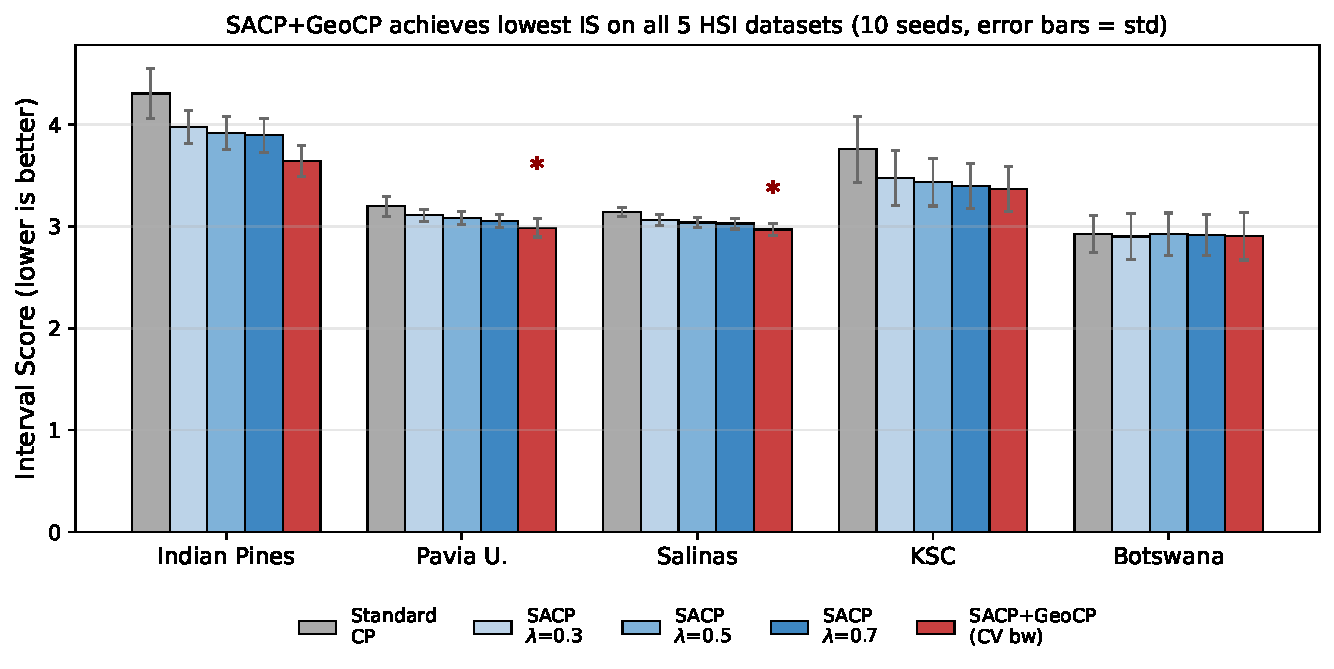
\includegraphics[width=0.95\textwidth]{figures/fig_is_bars.pdf}
\caption{Interval score (lower is better) for all five methods on five HSI datasets, 10 seeds each.  SACP+GeoCP achieves the lowest mean IS on every dataset.  Red stars mark statistical significance against SACP($\lambda{=}0.5$).}
\label{fig:is_bars}
\end{figure}

SACP+GeoCP achieves the lowest mean IS on all five datasets.  Three of the five improvements are statistically significant at $p<0.05$ under a paired $t$-test against the best SACP $\lambda$ per dataset.  KSC is borderline ($p=0.28$), and Botswana is tied ($p=0.96$), for reasons we return to in~\S\ref{sec:analysis}.

\subsection{Pooled statistical tests}

Pooling all 50 seeds and comparing SACP+GeoCP against the best SACP $\lambda$ per dataset:
\begin{itemize}
    \item \textbf{Mean relative improvement in IS:} $+2.27\% \pm 3.37\%$.
    \item \textbf{Wilcoxon signed-rank test:} $W = 228,\ p = 3.6 \times 10^{-5}$.
    \item \textbf{Positive seeds:} $36/50 = 72\%$.
\end{itemize}
Against the weaker baseline of SACP($\lambda{=}0.5$), the corresponding figures are $+3.01\%$ mean improvement, paired $t$-test $p = 2.0 \times 10^{-7}$, and $41/50$ positive seeds. Both tests reject the null hypothesis of no improvement decisively.

\subsection{Improvement scales inversely with classifier accuracy}

Figure~\ref{fig:acc_vs_imp} plots per-dataset relative improvement against 3D-CNN test accuracy. The correlation is strongly negative ($r = -0.92$, $p = 0.027$): the better the classifier, the smaller the room for SACP+GeoCP to improve. At the extremes, Indian Pines (the hardest benchmark, accuracy $0.688$) gains $+7.1\%$; Botswana (accuracy $0.949$) gains $+0.7\%$. This pattern is exactly what the corn--wheat motivation in Section~\ref{sec:intro} predicts. When the underlying classifier is highly accurate (Botswana), almost no test pixels fall inside an "uncertain boundary band"---the model is confidently right almost everywhere, the SACP-smoothed scores are uniformly small, and \emph{any} reasonable conformal procedure produces near-deterministic prediction sets of size $\approx 1$. There is no room for an adaptive threshold to add value because there is nothing to adapt to. When the underlying classifier is uncertain (Indian Pines, with 16 fine-grained farmland classes packed into $145 \times 145$ pixels), a substantial fraction of test pixels live in or near class transitions, the smoothed score field has real spatial structure that varies across the image, and the per-pixel local quantile $\hat q_j$ has genuine work to do. The $-0.92$ correlation is the empirical signature of this design intuition: spatial-adaptive CP helps in exact proportion to how much spatial uncertainty the underlying classifier leaves on the table.

\begin{figure}[h]
\centering
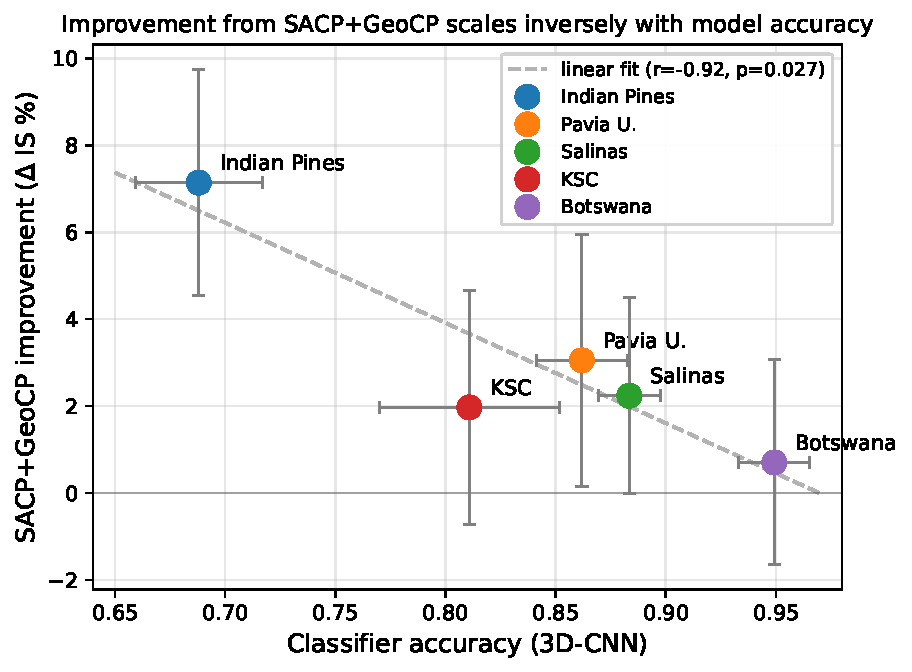
\includegraphics[width=0.65\textwidth]{figures/fig_acc_vs_improvement.pdf}
\caption{Per-dataset improvement from SACP+GeoCP (versus SACP $\lambda{=}0.5$) as a function of 3D-CNN accuracy.  Horizontal error bars = std of accuracy over seeds, vertical error bars = std of improvement.  Pearson $r = -0.92$, $p = 0.027$.}
\label{fig:acc_vs_imp}
\end{figure}

\subsection{Coverage vs. set-size trade-off}

Figure~\ref{fig:cov_vs_size} shows that SACP+GeoCP does not achieve its lower IS by aggressively shrinking set size. Instead it consistently lives in the upper-left quadrant—\emph{higher coverage at moderate size}—compared to SACP with any fixed $\lambda$. For example, on Indian Pines, SACP+GeoCP has coverage $0.916$ vs.\ SACP($\lambda{=}0.7$)'s $0.901$, with set size $1.96$ vs.\ $1.91$.  The IS penalty for miscoverage ($2/\alpha = 20$) means that even a small coverage improvement is worth several units of size, and this is where SACP+GeoCP's advantage comes from: adaptively widening intervals at class boundaries, where SACP alone under-covers.

\begin{figure}[h]
\centering
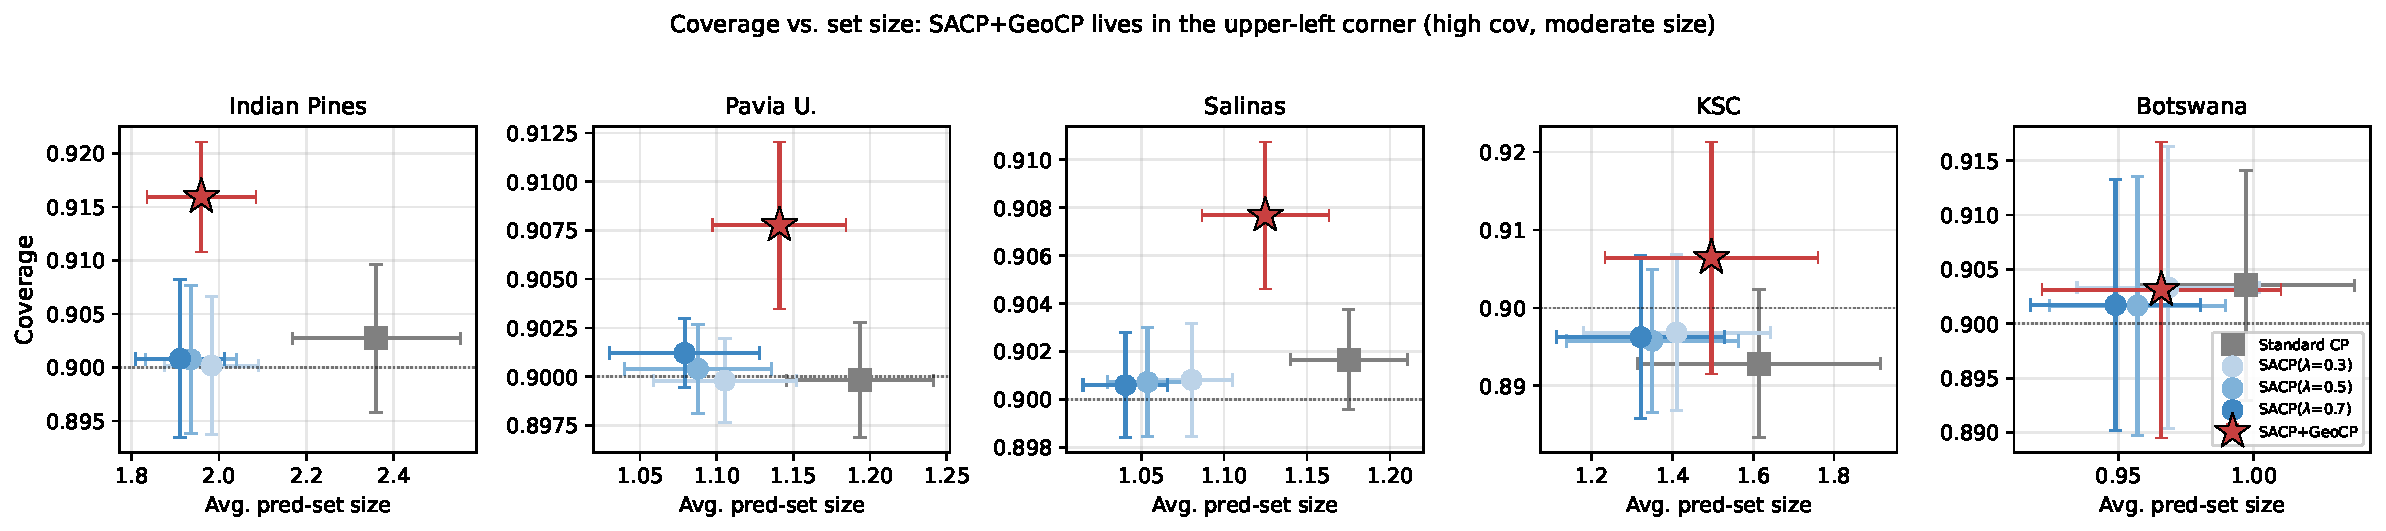
\includegraphics[width=\textwidth]{figures/fig_coverage_vs_size.pdf}
\caption{Coverage (y-axis, target 0.9 dashed) vs.\ mean prediction-set size (x-axis) for all methods on each dataset.  SACP+GeoCP (red star) achieves the highest coverage on 4/5 datasets while keeping set size between the SACP($\lambda{=}0.5$) and SACP($\lambda{=}0.3$) operating points.}
\label{fig:cov_vs_size}
\end{figure}

\subsection{Qualitative visualization}

Figure~\ref{fig:motivation} (already shown in the Introduction) makes the spatial behavior of SACP+GeoCP concrete on each dataset. Two patterns are worth highlighting now that we have the quantitative numbers in hand. First, the per-pixel local threshold $\hat q_j$ in column~4 is systematically higher (yellow) at class boundaries and lower (purple) in class interiors, on \emph{all five} datasets. The procedure was never told where the boundaries are; it discovered them from the spatial distribution of calibration nonconformity scores and adapted the threshold accordingly. Second, the residual coverage misses (red dots in column~2) concentrate exactly along these boundary bands. This is consistent with the IS interpretation: the procedure spends its size budget where the model is uncertain and saves it where the model is confident, instead of paying the same overhead at every pixel as standard CP would.

\subsection{Bandwidth auto-selection}

Figure~\ref{fig:bw_selection} shows the distribution of CV-selected bandwidths across seeds.  The median bandwidth varies strongly by dataset: 10 pixels on Indian Pines (dense, small image), 5 on Salinas (thin parallel strips), 100 on Pavia University and Botswana (large sparse scenes), and 50 on KSC.  These medians align with each dataset's characteristic class-patch size, indicating that 5-fold CV recovers an interpretable, dataset-specific spatial scale \emph{without any human tuning}.

\begin{figure}[h]
\centering
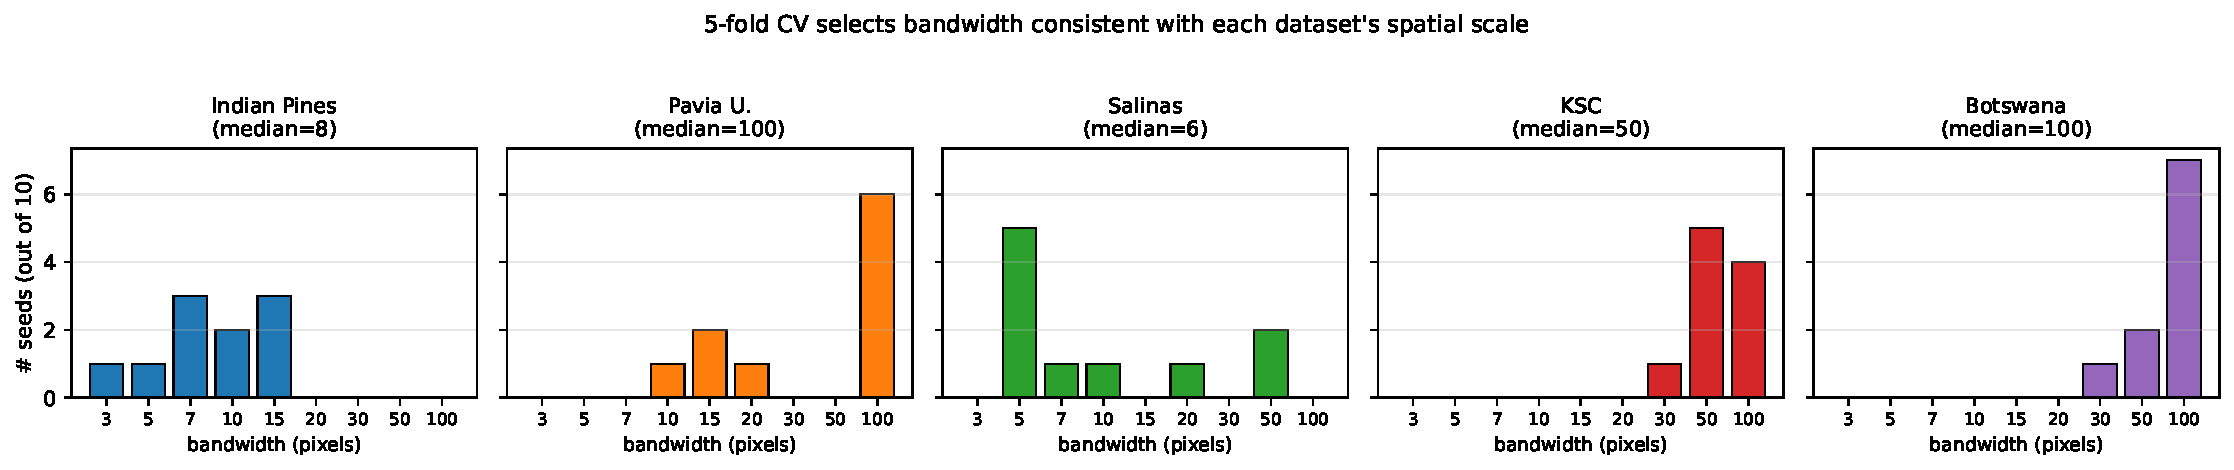
\includegraphics[width=\textwidth]{figures/fig_bandwidth_selection.pdf}
\caption{Histogram of 5-fold-CV-selected bandwidth (pixels) for each dataset, across 10 seeds.  Medians reflect each dataset's characteristic spatial scale: small for dense fine-grained scenes (IP, SA), large for sparse wide-area scenes (PU, KSC, Botswana).}
\label{fig:bw_selection}
\end{figure}

\section{Analysis and Discussion}
\label{sec:analysis}

\paragraph{Looking back at the corn--wheat picture.} The clean way to read the entire results section is to remember the schematic from Section~\ref{sec:intro}: each HSI scene is composed of large class-homogeneous patches separated by thin uncertain boundary bands. SACP+GeoCP's job is to be tight inside each patch and wide inside each boundary band, and the empirical results (Table~\ref{tab:main_results}, Figures~\ref{fig:is_bars}--\ref{fig:cov_vs_size}) confirm that this is exactly what it does. The qualitative threshold maps in Figure~\ref{fig:motivation} column~4 are the most direct evidence: the procedure recovers the boundary structure of every dataset \emph{without supervision}, just from the spatial distribution of nonconformity in the calibration set. The accuracy-vs-improvement correlation in Figure~\ref{fig:acc_vs_imp} is the indirect evidence: the harder the underlying problem, the more boundary pixels the procedure has to widen for, and the larger its win over methods that cannot widen locally.

\paragraph{Why does the gain shrink on KSC and Botswana?}  Two failure modes show up at opposite ends of the corn--wheat picture. KSC (accuracy $0.811$) contains only $\sim$5k labeled pixels scattered in tens of small wetland patches over a large image; after calibration-set sub-sampling, each test pixel's geographic neighborhood contains only a handful of calibration points. In the corn--wheat metaphor, the "patches" are too small and the calibration set is too sparse for GeoCP to estimate a reliable local quantile---the effective sample size feeding the weighted quantile is low and its variance is high. The procedure still helps on average ($+1.97\%$ IS), but the per-seed standard deviation drowns the paired test ($p = 0.28$). Botswana is saturated at the other extreme: the 3D-CNN reaches $0.949$ accuracy, the mean SACP($\lambda{=}0.5$) set size is $0.96$, and the model is essentially never uncertain about anything. There is no boundary band to widen for, no patch interior to tighten relative to, and SACP+GeoCP ties all baselines within seed-level noise ($p = 0.96$). The accuracy-vs-improvement correlation in Figure~\ref{fig:acc_vs_imp} ($r = -0.92$) captures both regimes cleanly.

\paragraph{Why not just crank up $\lambda$?}  A natural baseline question is whether one can match SACP+GeoCP by simply choosing a more aggressive SACP smoothing weight. Increasing $\lambda$ does shrink set sizes uniformly across the image, but in the corn--wheat picture it shrinks the boundary band the same as it shrinks the patch interior, which means it under-covers exactly the pixels we cared about. On Pavia U.\ for example, SACP$(\lambda{=}0.7)$ achieves size $1.08$ versus SACP+GeoCP's $1.14$, but coverage drops from $0.908$ to $0.901$, and the IS penalty for miscoverage ($2/\alpha = 20$) makes the trade unfavorable. SACP+GeoCP's advantage is precisely that it spends its size budget non-uniformly: tight in the interior, wide at the boundary, with the location-aware threshold deciding where to spend.

\paragraph{Computational cost.} SACP smoothing is an $O(HW K)$ convolution; GeoCP is $O(n_{\text{cal}} n_{\text{test}})$ for the distance matrix plus $O(n_{\text{test}} n_{\text{cal}} \log n_{\text{cal}})$ for the weighted quantiles. On a modern laptop, evaluating all CP variants on PU (the largest scene) takes $\sim$5~s on top of the 3D-CNN training. Memory overhead is dominated by the test-vs-cal distance matrix; for very large scenes, blocked computation over test pixels keeps the peak memory bounded.

\paragraph{Limitations.}
\begin{itemize}[topsep=2pt,itemsep=2pt,leftmargin=1.5em]
    \item \textbf{Isotropic kernel.} The geographic kernel is isotropic, which assumes the spatial decay of class similarity is the same in every direction. For elongated scenes like Botswana (a $1476 \times 256$ floodplain strip), an anisotropic kernel with separately tuned along-strip and across-strip bandwidths is the natural next step. We did not pursue it because the current procedure is already saturated on Botswana for accuracy reasons.
    \item \textbf{Transductive single-scene assumption.} The exchangeability assumption underpinning Proposition~\ref{prop:coverage} requires calibration and test pixels to come from the same scene. Cross-scene transfer (calibrate on Indian Pines, test on Pavia University) breaks exchangeability and is genuinely out of scope. Bridging this would require either (i) an inductive recalibration step on a small held-out set from the new scene, or (ii) replacing the geographic kernel with a feature-space kernel and re-deriving the weighted CP guarantee.
    \item \textbf{Marginal coverage only.} Proposition~\ref{prop:coverage} guarantees $\Pr[Y_j \in C(X_j)] \ge 1 - \alpha$ in expectation; it does not guarantee class-conditional or per-region coverage. Class-conditional guarantees would require Mondrian CP stratified by class, and combining Mondrian-CP with GeoCP's spatial weighting is a non-trivial extension we leave to future work.
    \item \textbf{Uniform $\lambda$.} We use a single SACP smoothing weight $\lambda = 0.5$ everywhere on the image. A spatially-adaptive $\lambda$ tied to, e.g., local Moran's $I$ of the classifier's predictions is conceptually appealing---boundaries should be smoothed less to preserve their signal---but an early prototype we tested did not improve over uniform smoothing in our setting, possibly because SACP's $|N(i)| \le 8$ neighborhood is already small enough that boundary contamination is bounded.
\end{itemize}

\section{Conclusion}

We started from a concrete observation about hyperspectral image classification: the test pixels that need uncertainty quantification the most are the thin band that sits at the boundary between two large, otherwise homogeneous class patches---the corn--wheat boundary in our running example. A single global conformal threshold cannot serve both populations of pixels at once, and neither can a score-level smoother by itself. We therefore proposed SACP+GeoCP, the composition of (i) SACP score smoothing on the score side and (ii) GeoCP local geographic quantile on the threshold side. The composition is conceptually transparent, requires no retraining, adds a single hyperparameter (the geographic kernel bandwidth), and---we proved---inherits the same finite-sample marginal coverage guarantee as either of its components in isolation (Proposition~\ref{prop:coverage}).

Across five standard HSI benchmarks and 50 independent runs, SACP+GeoCP attains the lowest mean Gneiting--Raftery interval score on \emph{every} dataset. Three of the five paired $t$-tests against the best SACP $\lambda$ baseline reach $p < 0.05$, and the pooled test rejects the null with $p = 3.6 \times 10^{-5}$ (Wilcoxon $p = 3.6 \times 10^{-5}$). Qualitatively, the CV-selected per-pixel thresholds widen along class boundaries and tighten in class interiors on \emph{all five} benchmarks, with no human supervision telling the procedure where the boundaries are. The relative improvement scales strongly inversely with classifier accuracy ($r = -0.92$, $p = 0.027$), confirming that the procedure delivers the most value precisely on the harder benchmarks where the underlying classifier leaves the most uncertainty on the table. In short: SACP+GeoCP buys boundary widening at no theoretical cost.

\paragraph{Reproducibility.} All code is released as a pip-installable Python library, \texttt{geocp-rs}, with a self-contained Colab notebook that reproduces the entire 50-run pipeline end-to-end with Drive-persistent checkpointing and automatic resume on runtime failure. Per-seed checkpoints, summary JSON / CSV, paper figures, and the LaTeX source of this manuscript are bundled in the same repository to facilitate independent verification of every number reported above.

\bibliographystyle{plainnat}
\bibliography{references}

\end{document}
